\documentclass{beamer}
\usepackage{multicol}
\usepackage{graphicx}
\usepackage{tikz}
\usepackage{tikzscale}
\usepackage[english]{babel}
\usepackage{amsmath}
\usepackage{amssymb}
\usepackage{mathtools}
\usepackage{mathrsfs}
\usepackage{xcolor}
\usepackage{physics}
\usepackage{bm}
\usepackage{bbm}
\usetheme[alternativetitlepage=bild]{Rub}
\newcommand{\I}{\mathbbm{i}}
\renewcommand{\vec}[1]{\bm{#1}}
\begin{document}
\title{Gaussian Random Field Generation \\for Stochastic PDEs}   
\author{Timo Schorlepp} 
\date{\today} 
\titlegraphic{titel.png}
\frame{\titlepage} 

\frame{\frametitle{Table of contents}\tableofcontents} 

%%%%%%%%%%%%%%%%%%%%%%%%%%%%%%%%%%%%%%%%%%%%%%%%%
\section{Motivation} 
%%%%%%%%%%%%%%%%%%%%%%%%%%%%%%%%%%%%%%%%%%%%%%%%%
\frame{\frametitle{Motivation:\\Exemplary applications} 
\begin{columns}[t]
\column{.5\textwidth}
\centering
\includegraphics[width=.65\textwidth]{figures/cosmogrf}\\
\tiny{
Vogelsberger et al. 2014, Illustris simulation}\\
\includegraphics[width=.65\textwidth]{figures/2dns}\\
\tiny{Murray 2017, 2$d$ stochastic NSE vorticity}
\column{.5\textwidth}
\centering
\includegraphics[width=.65\textwidth]{figures/kpz}\\
\tiny{Kuennen, Wang 2008, KPZ surface growth}\\[.2cm]
\includegraphics[width=.65\textwidth]{figures/aquifer}\\
\tiny{Wikimedia, aquifer sketch}
\end{columns}
}
%%%%%%%%%%%%%%%%%%%%%%%%%%%%%%%%%%%%%%%%%%%%%%%%%
\frame{\frametitle{Motivation:\\Mathematical examples} 
Deterministic incompressible NSE for $\vec{u}:\mathbb{T}^d \times \mathbb{R}_+ \to \mathbb{R}^d$:
\begin{align*}
\partial_t \vec{u} + (\vec{u} \cdot \nabla) \vec{u} + \nabla p = \nu \Delta \vec{u}\; , \; \nabla \cdot \vec{u} = 0 
\end{align*}
Without forcing: 
\begin{align*}
\dv{}{t} \int \mathrm{d}V \; \frac{1}{2} \abs{\vec{u}}^2 = - 2 \nu \int \mathrm{d}V \; \trace((\nabla \otimes \vec{u})^T (\nabla \otimes \vec{u})) \leq -2 C \nu \int \mathrm{d}V \; \abs{\vec{u}}^2
\end{align*}
Gronwall: Energy decays exponentially, need forcing for interesting long-term behavior, e.g. Gaussian forcing with homogeneous, isotropic correlation matrix!\\
\medskip
Similarly: Stochastic heat equation\\
Why Gaussian? CLT, easy, approximation, algorithms exist
}
%%%%%%%%%%%%%%%%%%%%%%%%%%%%%%%%%%%%%%%%%%%%%%%%%
\section{Theory} 
%%%%%%%%%%%%%%%%%%%%%%%%%%%%%%%%%%%%%%%%%%%%%%%%%
\subsection{Basic Definitions}
%%%%%%%%%%%%%%%%%%%%%%%%%%%%%%%%%%%%%%%%%%%%%%%%%
\frame{\frametitle{Theory:\\Basic Definitions}
\begin{block}{Definition 1}
A random field $\vec{\xi}$ is an indexed family of random variables
\begin{align*}
\vec{\xi} = \left\{ \vec{\xi}(\vec{x}) : \Omega \to \mathbb{R}^m \; ; \; \vec{x} \in T \subseteq \mathbb{R}^d \right\}.
\end{align*}
\end{block}
\begin{alertblock}{Remark 2}
\begin{itemize}
\item Generalization of stochastic processes
\item No details on Kolmogorov Existence Theorem etc. here
\end{itemize}
\end{alertblock}
}
%%%%%%%%%%%%%%%%%%%%%%%%%%%%%%%%%%%%%%%%%%%%%%%%%
\frame{\frametitle{Theory:\\Basic Definitions}
\begin{block}{Definition 3}
A random field $\vec{\xi}$ is called Gaussian iff $\forall k \in \mathbb{N}: \forall \{\vec{x}^{(0)}, \cdots , \vec{x}^{(k-1)} \} \subseteq T: \vec{\xi}(\vec{x}^{(0)}) =: \vec{\xi}^{(0)}, \cdots \vec{\xi}(\vec{x}^{(k-1)})=: \vec{\xi}^{(k-1)}$ are jointly normally distributed, i.e.
\begin{align*}
p_{\vec{\xi}^{(0)}, \cdots ,\vec{\xi}^{(k-1)}}(\vec{y}^{(0)}, \cdots \vec{y}^{(k-1)}) = &\det(2 \pi \Sigma)^{- \frac{1}{2}} \cdot \\ & \cdot \exp(-\frac{1}{2} (\vec{y}-\vec{\mu})^T \Sigma^{-1} (\vec{y}-\vec{\mu}))
\end{align*}
where $\Sigma$ is the $km \times km$ covariance matrix 
\begin{align*}
\Sigma_{m r + i,m s + j} = \text{Cov}\left(\xi^{(r)}_i,\xi^{(s)}_j \right) =: \chi_{ij}\left(\vec{x}^{(r)}, \vec{x}^{(s)} \right)
\end{align*}
and $\vec{\mu}$ is the $km$-dim.\ mean vector $\mu_{mr + i} = \left< \xi^{(r)}_i \right>$.
\end{block}
}
%%%%%%%%%%%%%%%%%%%%%%%%%%%%%%%%%%%%%%%%%%%%%%%%%
\frame{\frametitle{Theory:\\Basic Definitions}
\begin{alertblock}{Remark 4}
\begin{itemize}
\item Gaussian random fields (GRF) are completely specified by $\vec{\mu}(\vec{x})$ and $\chi \left(\vec{x}',\vec{x}\right)$ $\Longrightarrow$ easy!
\item We will assume $\vec{\mu}(\vec{x}) \equiv 0$ wlog in the following (also necessary for isotropy) as well as $d=m$
\item $\Sigma$ needs to be positive semidefinite for all $\vec{x}^{(0)},\cdots, \vec{x}^{(k-1)}$ since $\sum_{i,j}\vec{a}_i^T \chi \left(\vec{x}^{(i)},\vec{x}^{(j)}\right) \vec{a}_j = \text{Var}\left(\sum_{i} \vec{a}_i^T \vec{\xi}^{(i)} \right)\geq 0$\\
\end{itemize}
\end{alertblock}
}
%%%%%%%%%%%%%%%%%%%%%%%%%%%%%%%%%%%%%%%%%%%%%%%%%
\frame{\frametitle{Theory:\\Basic Definitions}
\begin{exampleblock}{Example/Definition 5}
\begin{itemize}
\item White noise $\chi_{ij}\left(\vec{x}',\vec{x}\right) = \delta(\vec{x}'-\vec{x}) \delta_{ij}$
\item Homogeneous (translation-invariant, stationary), isotropic ($O(n)$-invariant) and solenoidal correlation tensor:
\begin{align*}
\chi_{ij}(\vec{x}', \vec{x}) = \chi_{ij}(\vec{x}'-\vec{x}) = \chi_{ij}(\vec{r}) = f(r) \delta_{ij} + \frac{r f'(r)}{d-1} \left( \delta_{ij}-\frac{r_i r_j}{r^2}\right)
\end{align*}
\item Stationary diagonal correlation $\chi_{ij}(\vec{x}',\vec{x}) = \chi_0 \exp(-\frac{\abs{\vec{x}'-\vec{x}}}{\lambda}) \delta_{ij}$
\end{itemize}
\end{exampleblock}
\begin{alertblock}{Remark 6}
We do not distinguish between correlation and covariance matrices here (they differ by a constant factor in the stationary case)
\end{alertblock}
}
%%%%%%%%%%%%%%%%%%%%%%%%%%%%%%%%%%%%%%%%%%%%%%%%%
\subsection{How to generate stationary GRFs}
%%%%%%%%%%%%%%%%%%%%%%%%%%%%%%%%%%%%%%%%%%%%%%%%%
\frame{\frametitle{Theory:\\How to generate stationary GRFs}
\begin{exampleblock}{Example 7}
Assuming we can generate independent $\mathcal{N}(0,1)$ samples, how do we generate vectors $\vec{\xi} \sim \mathcal{N}(0,C)$ for a given covariance $d \times d$-matrix $C$?\\
\medskip
Answer: $C$ is positive semidefinite, allowing for a Cholesky or eigenvalue/-vectors decomposition $C=B^T B$, so if we sample $\vec{\phi}$ with independent $\mathcal{N}(0,1)$ entries, we get
\begin{align*}
\left< B^T \vec{\phi} \;  (B^T \vec{\phi})^T \right> = B^T \underbrace{\left< \vec{\phi} \vec{\phi}^T \right>}_{=I_d} B = B^T B = C
\end{align*}
\end{exampleblock}
}
%%%%%%%%%%%%%%%%%%%%%%%%%%%%%%%%%%%%%%%%%%%%%%%%%
\frame{\frametitle{Theory:\\How to generate stationary GRFs}
\begin{block}{Theorem 8 (Direct method)}
Let 
\begin{align*}
G = \left\{ \left( j_1 \frac{L_1}{N_1} , \cdots , j_d \frac{L_d}{N_d} \right) \; ; j_s \in \{ 0 , 1 , 2 , \cdots , N_s - 1   \} \right\}
\end{align*}
be a uniformly spaced grid in $[0,L_1] \times \cdots \times [0,L_d]$. Decomposing the overall $(N_1 \cdots N_d d) \times (N_1 \cdots N_d d)$ grid covariance matrix $\Sigma = \Lambda^T \Lambda$ of the grid and sampling $\vec{\phi} \sim \mathcal{N}(0,I_{N_1 \cdots N_d d})$ yields
\begin{align*}
\Lambda^T \vec{\phi} \sim \mathcal{N}(0,\chi)
\end{align*}
\end{block}
\begin{alertblock}{Remark 9}
Decomposing this matrix becomes prohibitively expensive really fast!
\end{alertblock}
}
%%%%%%%%%%%%%%%%%%%%%%%%%%%%%%%%%%%%%%%%%%%%%%%%%
\frame{\frametitle{Theory:\\How to generate stationary GRFs}
\begin{exampleblock}{Example 10}
Grid covariance matrix for stationary $\chi$ on $2D$ $8 \times 8$ grid:
\centering
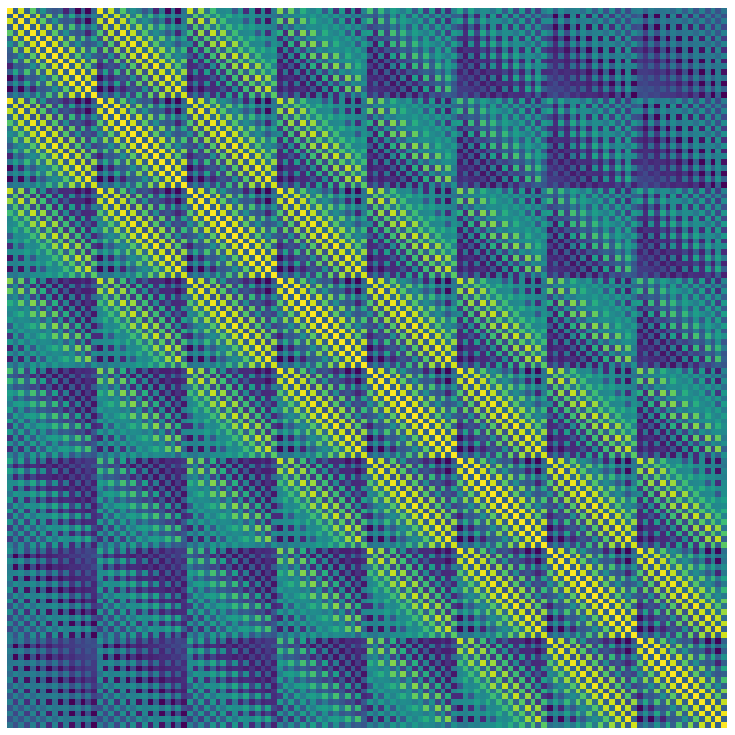
\includegraphics[width=.45\textwidth]{figures/bttb}\\
Block Toeplitz matrix (BTM)
\end{exampleblock}
}
%%%%%%%%%%%%%%%%%%%%%%%%%%%%%%%%%%%%%%%%%%%%%%%%%
\frame{\frametitle{Theory:\\How to generate stationary GRFs}
\begin{exampleblock}{Example 10 (continued, circulant embedding)}
Idea: Embed the BTM into a block \textit{circulant} matrix (BCM) by extending the grid with periodic boundary conditions. Goal: Use properties of BCMs (eigenvalues may be found via FFT of the individual $d \times d$ blocks)\\
\centerline{
\includegraphics[width=0.44\textwidth]{figures/embedgrd}
}
\end{exampleblock}
}
%%%%%%%%%%%%%%%%%%%%%%%%%%%%%%%%%%%%%%%%%%%%%%%%%
\frame{\frametitle{Theory:\\How to generate stationary GRFs}
\begin{alertblock}{Remark 11 (circulant embedding)}
\begin{itemize}
\item The extended covariance matrix need not be positive (semi)definite!\\
$\Longrightarrow$ Grid may need to be very large  
\item No further details here, check the literature list on last slide if you are interested in circulant embedding methods
\end{itemize}
\end{alertblock}
}
%%%%%%%%%%%%%%%%%%%%%%%%%%%%%%%%%%%%%%%%%%%%%%%%%
\frame{\frametitle{Theory:\\How to generate stationary GRFs}
\begin{block}{Theorem 12 (Spectral method, continuous FT)}
Let $\vec{\xi}$ be a stationary GRF on $\mathbb{R}^d$ with correlation matrix $\chi$. Denote by $\vec{W}$ the $d$-dimensional white noise $\langle \vec{W}(\vec{x}') \vec{W}(\vec{x})^T \rangle = I_d \; \delta(\vec{x}'-\vec{x})$, and by $\mathscr{F}$ the Fourier transform (FT) on $\mathbb{R}^d$. Decompose the correlation in Fourier space as $\hat{\chi}(\vec{k}) := \mathscr{F} \chi(\vec{k}) = \Lambda(\vec{k}) \Lambda^\dagger(\vec{k})$. Then, the following statements hold:\\
\begin{enumerate}
\item $\vec{\psi} := (\mathscr{F}^{-1} \Lambda \mathscr{F}) \;\vec{W} \stackrel{\mathcal{D}}{=} \vec{\xi}$.
\item $\hat{\vec{W}}$ has covariance $\left< \hat{\vec{W}}(\vec{k}')\hat{\vec{W}}(\vec{k})^\dagger \right> = (2 \pi)^d I_d \; \delta(\vec{k}' -\vec{k})$ and pseudo-covariance $\left< \hat{\vec{W}}(\vec{k}') \hat{\vec{W}}(\vec{k})^T \right> = (2 \pi)^d I_d \; \delta(\vec{k}' + \vec{k})$.
\item $\hat{\vec{\xi}}$ has covariance $\left< \hat{\vec{\xi}}(\vec{k}')\hat{\vec{\xi}}(\vec{k})^\dagger \right> = (2 \pi)^d \hat{\chi}(\vec{k}) \; \delta(\vec{k}' -\vec{k})$ and pseudo-covariance $\left< \hat{\vec{\xi}}(\vec{k}') \hat{\vec{\xi}}(\vec{k})^T \right> = (2 \pi)^d \hat{\chi}(\vec{k}) \; \delta(\vec{k}' + \vec{k})$.
\end{enumerate}
\end{block}
}
%%%%%%%%%%%%%%%%%%%%%%%%%%%%%%%%%%%%%%%%%%%%%%%%%
\frame{\frametitle{Theory:\\How to generate stationary GRFs}
\small
\textbf{Proof}: (1) Standard computation
\begin{align*}
&\langle \vec{\psi}(\vec{x}') \vec{\psi}(\vec{x})^\dagger \rangle = \biggl< \frac{1}{(2 \pi)^{d}} \int \mathrm{d}^d k' e^{\I \vec{k}' \cdot \vec{x}'} \Lambda(\vec{k}') \int \mathrm{d}^d y' e^{-\I \vec{k}' \cdot \vec{y}'} \vec{W}(\vec{y}') \\
& \quad \cdot \frac{1}{(2 \pi)^d} \int \mathrm{d}^d y \vec{W}(\vec{y})^T e^{\I \vec{k} \cdot \vec{y}} \int \mathrm{d}^d k \; \Lambda(\vec{k})^\dagger e^{- \I \vec{k} \cdot \vec{x}} \biggr> \\
&= \frac{1}{(2 \pi)^{2d}} \int \mathrm{d}^d k' \int \mathrm{d}^d k  \int \mathrm{d}^d y'  \int \mathrm{d}^d y 
\; e^{\I \vec{k}' \cdot (\vec{x}'-\vec{y}')+ \I \vec{k} \cdot (\vec{y} - \vec{x})}\\
& \quad \cdot \Lambda(\vec{k}') \underbrace{\langle \vec{W}(\vec{y}')   \vec{W}(\vec{y})^T \rangle}_{=I_d \delta(\vec{y}'-\vec{y})} \Lambda(\vec{k})^\dagger\\
&= \frac{1}{(2 \pi)^{d}} \int \mathrm{d}^d k' \int \mathrm{d}^d k   \underbrace{\frac{1}{(2 \pi)^{d}} \int \mathrm{d}^d y' e^{\I (\vec{k} - \vec{k}') \cdot \vec{y}'}}_{= \delta (\vec{k} - \vec{k}')}
\; e^{\I \vec{k}' \cdot \vec{x}' - \I \vec{k} \cdot \vec{x}}
\Lambda(\vec{k}') \Lambda(\vec{k})^\dagger \\
&= \frac{1}{(2 \pi)^{d}} \int \mathrm{d}^d k 
\; e^{\I \vec{k} \cdot (\vec{x}' - \vec{x})}
\underbrace{\Lambda(\vec{k}) \Lambda(\vec{k})^\dagger}_{= \hat{\chi}(\vec{k})} = \chi(\vec{x}'-\vec{x})
\end{align*}
}
%%%%%%%%%%%%%%%%%%%%%%%%%%%%%%%%%%%%%%%%%%%%%%%%%
\frame{\frametitle{Theory:\\How to generate stationary GRFs}
\small
\textbf{Proof}: (2) (and (3) analogously)
\begin{align*}
\left< \hat{\vec{W}}(\vec{k}')\hat{\vec{W}}(\vec{k})^\dagger \right> =
\int \mathrm{d}^d x' \int\mathrm{d}^d x e^{-\I \vec{k}' \cdot \vec{x}'} e^{\I \vec{k} \cdot \vec{x}}  \langle \vec{W}(\vec{x}') \vec{W}(\vec{x})^T \rangle = (2 \pi)^d I_d \; \delta(\vec{k}' -\vec{k})
\end{align*}
$\vec{W}$ is real $\Longrightarrow$ $\left< \hat{\vec{W}}(\vec{k}')\hat{\vec{W}}(\vec{k})^T \right> =(2 \pi)^d I_d \; \delta(\vec{k}' +\vec{k})$\\
\normalsize
\begin{alertblock}{Remark 13}
Theorem 11 shows that the Fourier modes of a stationary GRF are "decoupled" (modulo symmetry, due to $\vec{\xi}$ being real). Thus, instead of decomposing a $(N_1 \cdots N_d d) \times (N_1 \cdots N_d d)$ matrix, we need to decompose (analytically, so far) a single $d \times d$ matrix.
\end{alertblock}
}
%%%%%%%%%%%%%%%%%%%%%%%%%%%%%%%%%%%%%%%%%%%%%%%%%
\frame{\frametitle{Theory:\\How to generate stationary GRFs}
\begin{exampleblock}{Example 14}
Homogeneous, isotropic, solenoidal correlation tensor
\begin{align*}
\chi_{ij}(\vec{x}', \vec{x}) = \chi_{ij}(\vec{x}'-\vec{x}) = \chi_{ij}(\vec{r}) = f(r) \delta_{ij} + \frac{r f'(r)}{d-1} \left( \delta_{ij}-\frac{r_i r_j}{r^2}\right)
\end{align*}
with $f(r) := \chi_0 \, e^{-r^2/2\lambda^2}$ for $d=2$:
\begin{align*}
\chi(\vec r) &= \frac{\chi_0}{\lambda^2} \,
e^{-\frac{r^2}{2\lambda^2}} \, \left(\begin{array}{cc}
\lambda^2 - y^2 & x y \\
x y & \lambda^2 - x^2
\end{array}\right)\\ 
\Longrightarrow \hat{\chi}(\vec{k}) &= 2\pi \chi_0 \lambda^4 e^{-\frac{1}{2} k^2 \lambda^2} \,
\left(\begin{array}{cc}
k_y^2 & -k_x k_y\\
-k_x k_y & k_x^2
\end{array}\right)
\end{align*}
\end{exampleblock}
}
%%%%%%%%%%%%%%%%%%%%%%%%%%%%%%%%%%%%%%%%%%%%%%%%%
\section{Numerical implementation}
%%%%%%%%%%%%%%%%%%%%%%%%%%%%%%%%%%%%%%%%%%%%%%%%%
\frame{\frametitle{Numerical implementation}
What happens/changes if we want to apply the spectral method to generate GRF realizations on a grid in a bounded domain numerically, using the discrete fast Fourier transform (FFT)?\\
\begin{enumerate}
\item Sample discretized white noise: $\left< \vec{W}_i \vec{W}_j^T \right> = \frac{1}{\Delta_d}I_d \delta_{ij}\; ; \; \Delta_d := \frac{L_1 \cdots L_d}{N_1 \cdots N_d}$
\item Apply FFT to obtain discretized version of $\hat{\vec{W}}$ (alternatively: start in Fourier space, need to make sure though that symmetry is fulfilled!)
\item Multiply by $(2 \pi)^{d/2}\Lambda(\vec{k})$ which was calculated analytically via continuous FT on $\mathbb{R}^d$ (!)
\item Apply inverse FFT$/(2 \pi)^{d/2}$
\end{enumerate}
\textcolor{red}{$\Longrightarrow$ Conceptually, we start in Fourier space and impose the correlation $\hat{\chi}$ there! What kind of correlation do we obtain in real space if we use the discrete FT?}
}
%%%%%%%%%%%%%%%%%%%%%%%%%%%%%%%%%%%%%%%%%%%%%%%%%
\frame{\frametitle{Numerical implementation}
For simplicity: Consider $d=1$ and let
\begin{align*}
\varphi(x) = \sum_{m= -\infty}^{\infty} \chi(x + m L)
\end{align*} 
be the $L$-periodic summation of the initial correlation function $\chi$. Formally computing the Fourier transform yields
\begin{align*}
\hat{\varphi}(k) 
= \hat{\chi}(k) \sum_{m= -\infty}^{\infty} e^{\I k m L} = \frac{2 \pi}{L} \hat{\chi}(k) \sum_{m= -\infty}^{\infty} \delta(k - m\frac{2 \pi}{L})
\end{align*}
Applying the inverse FT:
\begin{align*}
\varphi(x) = \frac{1}{L} \sum_{m= -\infty}^{\infty} \hat{\chi} \left( m \frac{2 \pi}{L} \right) e^{2 \pi \I \frac{m}{L} x}
\end{align*}
}

\frame{\frametitle{Numerical implementation}
Using our algorithm (and notation $k_p = \frac{2 \pi}{L} p$):
\begin{align*}
\left<\xi_r \xi_s^\dagger \right> 
&= \frac{1}{N^2} \sum_{j,j',p,p'=0}^{N-1} e^{-\frac{2 \pi \I}{N} ( l j - p' j' + r p -  s p')} \Lambda(k_p) \underbrace{\left< W_p W_{p'}^T\right>}_{= N/L \; \delta_{jj'}} \Lambda(k_{p'})^\dagger \\
&= \frac{1}{N L} \sum_{j,p,p'=0}^{N-1} e^{-\frac{2 \pi \I}{N} j(p-p')} e^{\frac{2 \pi \I}{N}(sp'-rp)} \Lambda(k_p) \Lambda(k_{p'})^\dagger\\
&= \frac{1}{L} \sum_{p,p'=0}^{N-1} \delta_{pp'} e^{\frac{2 \pi \I}{N}(sp'-rp)}  \Lambda(k_p) \Lambda(k_{p'})^\dagger\\
&= \frac{1}{L} \sum_{p=0}^{N-1} \hat{\chi}(k_p) e^{\frac{2 \pi \I}{N} p (s-r)} \approx \varphi\left((s-r)\frac{L}{N}\right) = \varphi(x_s - x_r)
\end{align*}
}
%%%%%%%%%%%%%%%%%%%%%%%%%%%%%%%%%%%%%%%%%%%%%%%%%
\frame{\frametitle{Numerical implementation}
Example: $d=1$ and $\chi(r) = \chi_0 \, e^{-r^2/2\lambda^2}$
\medskip
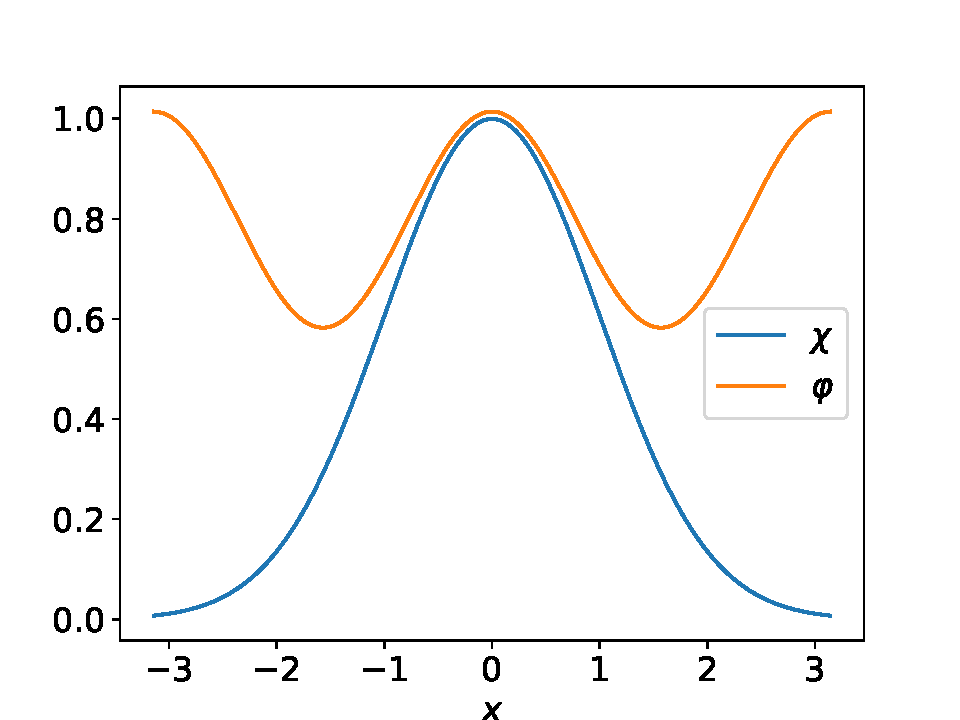
\includegraphics[width=.65\textwidth]{figures/chiphi}\\
\textcolor{red}{$\Longrightarrow$ Method only applicable if we use periodic boundary conditions in real space OR correlation length small + boundaries unimportant!}
}
\frame{\frametitle{Numerical implementation}
\textcolor{red}{Now}: Switch to source code!\\
We will see a concrete implementation of the algorithm and a demonstration of convergence of the covariance for increasing number of samples.
}
%%%%%%%%%%%%%%%%%%%%%%%%%%%%%%%%%%%%%%%%%%%%%%%%%
\section{Application to 1$d$ KPZ equation} 
\frame{\frametitle{Application to 1$d$ KPZ equation:\\Setup}
The evolution of the height $h$ of a growing interface may be modelled by the Kardar-Parisi-Zhang equation (1986):
\begin{align*}
\partial_t h = \nu \Delta h + \frac{\lambda}{2} \abs{\nabla h}^2 + \xi\\
\left<\xi(x',t') \xi(x,t) \right> = D \; \chi(x'-x) \delta(t'-t)
\end{align*}
where \textcolor{red}{$\chi(x'-x) = \delta(x'-x)$} in the classical KPZ equation.\\
In this case, for $d=1$ with a two-sided Wiener process as initial height profile, the stationary two-point correlation scales as
\begin{align*}
C(x,t) = \left<(h(x,t)-h(0,0)-t \langle \partial_t h\rangle)^2 \right> \propto t^{2/3} g\left( x t^{-2/3} \right)
\end{align*}
and in particular
\begin{align*}
C(0,t) \propto t^{2/3}.
\end{align*}
(Pr\"ahofer, Spohn 2004)
}
%%%%%%%%%%%%%%%%%%%%%%%%%%%%%%%%%%%%%%%%%%%%%%%%% 
\frame{\frametitle{Application to 1$d$ KPZ equation:\\Discretization}
Discretization using Heun scheme
\begin{align*}
h_n^{(1)} &= h_n(t_i) + \frac{\nu \Delta t}{(\Delta x)^2} \left[h_{n+1}(t_i)-2 h_n(t_i) + h_{n-1}(t_i) \right]\\
& \quad + \frac{\lambda \Delta t}{8 (\Delta x)^2} \left[h_{n+1}(t_i)-h_{n-1}(t_i) \right]^2 + \sqrt{\Delta t} \; \xi_{ni}\\
h_n(t_{i+1}) &= h_n(t_i) + \frac{\nu \Delta t}{2 (\Delta x)^2} \left[h_{n+1}(t_i)-2 h_n(t_i) + h_{n-1}(t_i) \right.\\
& \left. \quad + h_{n+1}^{(1)}-2 h_n^{(1)} + h_{n-1}^{(1)}\right]\\
& \quad +  \frac{\lambda \Delta t}{16 (\Delta x)^2} \left[ \left( h_{n+1}(t_i) - h_{n-1}(t_i) \right)^2 + \left( h_{n+1} - h_{n-1} \right)^2 \right]\\
& \quad +  \sqrt{\Delta t} \;  \xi_{ni}
\end{align*}
CFL: At least deterministic condition $\Delta t \leq (\Delta x)^2/(2 \nu)$ necessary!
}
%%%%%%%%%%%%%%%%%%%%%%%%%%%%%%%%%%%%%%%%%%%%%%%%%
\frame{\frametitle{Application to 1$d$ KPZ equation:\\Results}
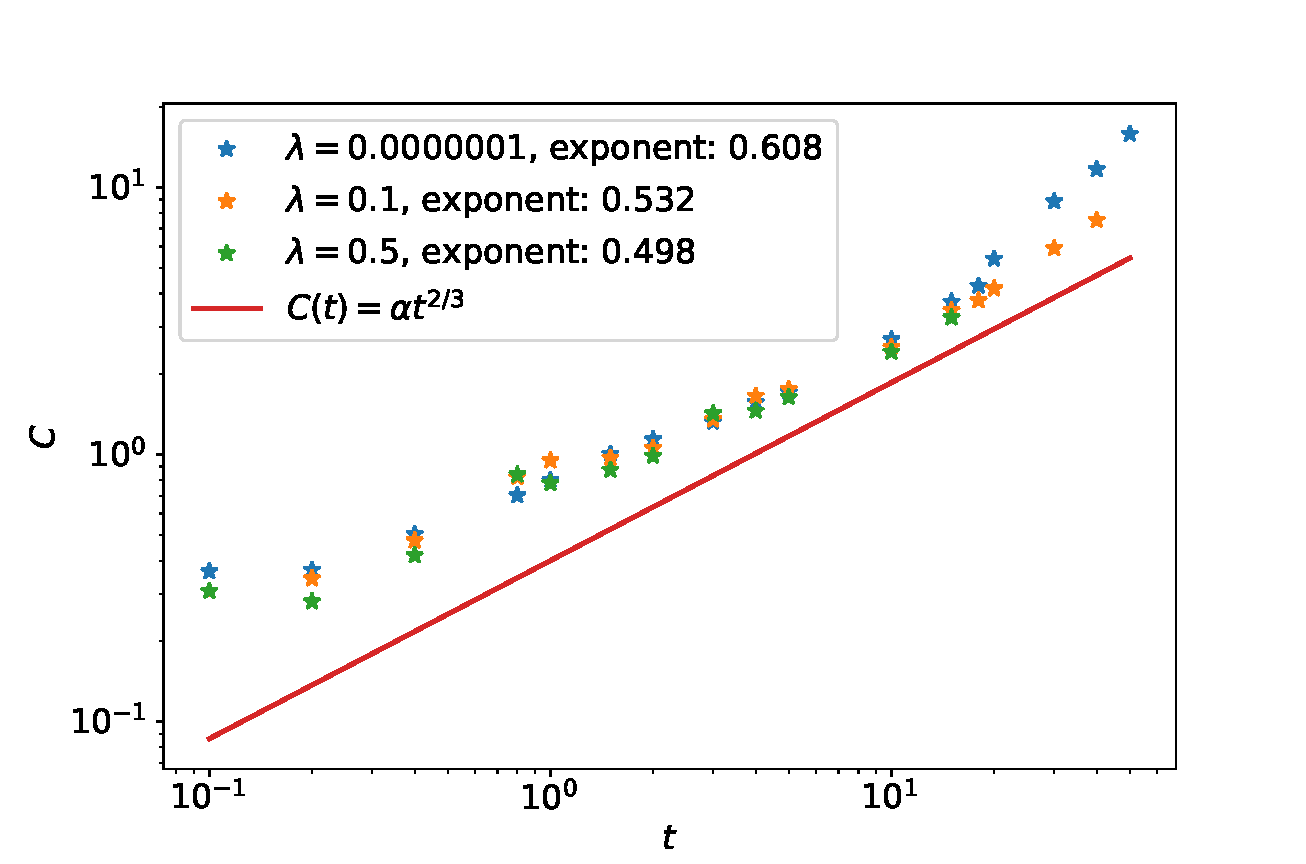
\includegraphics[width=0.8\textwidth]{figures/kpzresult}
}
%%%%%%%%%%%%%%%%%%%%%%%%%%%%%%%%%%%%%%%%%%%%%%%%%
\section{Conclusion}
%%%%%%%%%%%%%%%%%%%%%%%%%%%%%%%%%%%%%%%%%%%%%%%%%
\frame{\frametitle{Conclusion}
\begin{itemize}
\item Successfully sampled GRF realizations with stationary, isotropic and solneoidal correlation matrix
\item Used the FFT to avoid dealing with large grid covariance matrices, imposes periodic boundary conditions
\item Implemented a simple application for the 1$d$ KPZ equation, could investigate further
\item Other follow-ups: Implement and compare to circulant embedding, try different correlation matrices, application to stochastic NSE
\end{itemize}
}
%%%%%%%%%%%%%%%%%%%%%%%%%%%%%%%%%%%%%%%%%%%%%%%%%
\section{Literature}
%%%%%%%%%%%%%%%%%%%%%%%%%%%%%%%%%%%%%%%%%%%%%%%%%
\frame{\frametitle{Literature:\\Recommendations for further reading}
\begin{itemize}
\item A.\ Yaglom, Correlation Theory of Stationary and Related Random Functions, Springer Series in Statistics, 1987.
\item P.\ Abrahamsen, A Review of Gaussian Random Fields and Correlation Functions, Norsk Regnesentral/Norwegian Computing Center, 1997.
\item G.\ Chan, A.\ T.\ A.\ Wood, Simulation of stationary Gaussian vector fields, Statistics and Computing, 1999.
\item A.\ Lang, J.\ Potthoff, Fast simulation of Gaussian random fields, Monte Carlo Methods and Applications, 2011.
\item J.\ Carron, M.\ Wolk, I.\ Szapudi, On fast generation of cosmological random fields, MNRAS, 2014.
\end{itemize}
}
%%%%%%%%%%%%%%%%%%%%%%%%%%%%%%%%%%%%%%%%%%%%%%%%%
\frame{\frametitle{Literature:\\Recommendations for further reading}
\begin{itemize}
\item M.\ Kardar, G.\ Parisi, Y.\ Zhang, Dynamic Scaling of Growing Interfaces, Phys.\ Rev.\ Lett.\ , 1986
\item M.\ Pr\"ahofer, H.\ Spohn, Exact Scaling Functions for One-Dimensional Stationary KPZ Growth, Journal of Statistical Physics, 2004
\item S.\ Mathey et.\ al.\ , KPZ equation with short-range
correlated noise: emergent symmetries and non-universal
observables, Phys.\ Rev.\ E, 2016
\item R.\ Toral, P.\ Colet, Stochastic Numerical Methods: An Introduction for Students and Scientists, John Wiley \& Sons, 2014
\end{itemize}

}
\end{document}
 